\documentclass[conference]{IEEEtran}
\IEEEoverridecommandlockouts

\usepackage{cite}
\usepackage{amsmath,amssymb,amsfonts}
\usepackage{algorithmic}
\usepackage{algorithm}
% Unnumbered full-width header line inside algorithmic (for phase markers).
% Empty-label \item skips both the line number and the ALC@line counter,
% while inheriting the current block indent.
\makeatletter
\newcommand{\PHASE}[1]{\item[]{\normalfont\bfseries #1}}
\makeatother
\usepackage{graphicx}
\usepackage{subcaption}
\usepackage{textcomp}
\usepackage{xcolor}
\usepackage{blindtext}
\usepackage{stfloats}
\def\BibTeX{{\rm B\kern-.05em{\sc i\kern-.025em b}\kern-.08em
    T\kern-.1667em\lower.7ex\hbox{E}\kern-.125emX}}
\begin{document}

\title{PACE: Probabilistic Adaptive Contention Control for Non-Primary Channel Access in IEEE 802.11bn}

\author{
\IEEEauthorblockN{Taewon Song}
\IEEEauthorblockA{\textit{Division of Electronics and Electrical Engineering} \\
\textit{Dongguk University}\\
Seoul, Republic of Korea \\
twsong@dongguk.edu}
}

\maketitle

\begin{abstract}
Modern Wi-Fi deployments increasingly suffer from spectrum underutilization as overlapping Basic Service Sets (OBSSs) compete for primary channel access. IEEE 802.11bn introduces Non-Primary Channel Access (NPCA) to exploit these underutilized intervals, yet the standard contention mechanism is fundamentally mismatched to NPCA's constrained transmission windows: backoff counters routinely exceed the remaining opportunity duration, wasting slots that could otherwise carry data.
We propose PACE, a probabilistic adaptive contention control scheme that enables stations to collectively converge toward a theoretically optimal transmission probability without central coordination. PACE combines a distributed multiplicative feedback rule---copying the successful sender's probability on solo receptions---with a prospective self-exclusion mechanism that silences stations whose frame length exceeds the remaining window.
We evaluate PACE through simulation spanning a wide range of station counts and window lengths, comparing against Binary Exponential Backoff and several competing adaptive schemes under both homogeneous and heterogeneous frame-length distributions. PACE consistently outperforms standard backoff in channel utilization and achieves Pareto-dominance in the throughput--fairness tradeoff. The advantage is most pronounced when the available window is scarce relative to the contending population, precisely the regime in which standard backoff wastes the largest share of transmission opportunities.
These results identify the tight-window regime as the critical operating condition for NPCA and establish PACE as a practical design reference for adaptive contention policy in next-generation Wi-Fi networks.
\end{abstract}


\begin{IEEEkeywords}
Non-Primary Channel Access, IEEE 802.11bn, Probabilistic Access Control, OBSS, Adaptive Contention, Wi-Fi
\end{IEEEkeywords}

\IEEEpeerreviewmaketitle

% Introduction
\section{Introduction}
\label{sec:introduction}

Spectrum efficiency in next-generation Wi-Fi networks depends critically on how
effectively stations (STAs) exploit available channel time. In dense deployments, overlapping
Basic Service Sets (OBSSs) routinely occupy the primary channel while adjacent channels
remain idle, creating a persistent underutilization problem. IEEE 802.11bn addresses
this gap by introducing Non-Primary Channel Access (NPCA), which allows STAs to
transmit opportunistically on non-primary channels during ongoing OBSS intervals~\cite{ieee80211bn,wei2024non}.

NPCA, however, presents a contention challenge distinct from conventional channel
access. Each NPCA opportunity has a finite duration bounded by the ongoing OBSS
transmission, and competing STAs must coordinate their access within this
constrained window. The Binary Exponential Backoff (BEB) mechanism was designed for
open-ended contention: each collision doubles the backoff window, and the resulting
delay frequently exceeds the remaining NPCA window duration. Affected STAs are
effectively silenced for the rest of the interval, leaving the channel idle even when
other STAs could have transmitted. In heterogeneous deployments where STAs
carry frames of varying lengths, the problem is further compounded: STAs whose
frame cannot fit in the remaining window continue to occupy contention slots despite
having no viable transmission opportunity.

Consider a dense office environment where multiple STAs detect an OBSS transmission
and attempt to use the secondary channel concurrently. Early collisions trigger
exponential backoff growth; within a few rounds, a large fraction of STAs have
accumulated backoff counts that exceed the remaining window duration. The channel
spends the final slots idle, not because no STA wanted to transmit, but because
the contention mechanism pushed every backoff counter beyond the opportunity horizon.

Existing work on NPCA has focused on characterizing aggregate throughput and delay
under the standard switching rule, taking Binary Exponential Backoff within the
non-primary channel as given \cite{wei2024non,bellalta2025performance,wei2024optimized}.
The contention dynamics within the finite NPCA window---and the mismatch between
BEB's infinite-horizon design and the window's bounded duration---have not been
addressed. Adaptive probabilistic schemes designed for infinite-horizon neighbor
discovery, such as the ALOHA-like Neighbor Discovery (AND) algorithm
\cite{vasudevan2013efficient}, reduce overhead by avoiding explicit coordination,
but their stationary-population assumption makes them ill-suited to a window that
depletes over time. BEB's infinite-horizon design and AND's open-loop phase structure
both fail to track the time-varying optimal access probability as the window shrinks
and the set of viable STAs changes (see Table~\ref{tab:comparison}).

In this paper, we propose PACE, a Probabilistic Adaptive Contention control scheme
for NPCA that enables STAs to collectively converge toward the theoretically
optimal transmission probability for each moment within the window, without central
coordination or explicit inter-STA signaling. PACE adapts the MIMD feedback rule
of the Probabilistic Neighbor Discovery (PND) algorithm \cite{song2014pnd} to the
finite-window NPCA context: STAs copy the successful sender's probability on solo
receptions, reduce on collision, and increase on idle slots, causing distributed
dynamics to track the throughput-optimal policy. PACE further adds a
PPDU-aware self-exclusion rule that silences STAs whose frame length exceeds the
remaining window, eliminating a class of futile contention attempts that BEB would
otherwise sustain.

The design of PACE is motivated by two requirements that are unique to
NPCA's bounded-window structure: \textit{(i)} the optimal transmission
probability is time-varying and must track the depleting window rather than
converge to a static equilibrium, and \textit{(ii)} STAs whose frame
length exceeds the remaining window must proactively self-exclude to prevent
futile contention that wastes viable slots. The main contributions of this
paper are as follows:
\begin{itemize}
  \item We derive the throughput-optimal transmission probability for
        finite-window NPCA, showing that it must continuously track the
        remaining window duration and the number of still-viable competing
        STAs---a time-varying target that neither BEB nor existing
        infinite-horizon adaptive schemes can follow.
  \item We propose PACE, a fully distributed algorithm that addresses both
        requirements simultaneously: MIMD feedback drives the transmission
        probability toward the time-varying optimum~\textit{(i)}, while
        PPDU-aware self-exclusion eliminates futile contention by silencing
        STAs that cannot complete a frame within the remaining
        window~\textit{(ii)}, all without inter-STA signaling or
        knowledge of the total STA count.
  \item Through extensive simulation under homogeneous and heterogeneous
        frame-length distributions, we demonstrate that PACE achieves
        significantly higher window utilization than BEB, is Pareto-dominant
        in the throughput--fairness tradeoff, and maintains proportional
        fairness between native and visiting STAs.
\end{itemize}

\begin{table*}[ht]
\centering
\caption{Comparison of Contention Control Schemes}
\label{tab:comparison}
\begin{tabular}{lp{4cm} p{4cm}ccc}
\hline
\textbf{Method} & \textbf{Mechanism} & \textbf{Objective} & \textbf{PPDU-aware} & \textbf{Signaling-free} & \textbf{NPCA target} \\
\hline
AND~\cite{vasudevan2013efficient}           & Fixed-probability slotted ALOHA                            & Discover all neighbors in finite time without coordination    & $\times$   & \checkmark & $\times$   \\ \hline
PND~\cite{song2014pnd}                      & Multiplicative feedback with solo-copy rule                & Converge transmission probability to optimal without $N$      & $\times$   & \checkmark & $\times$   \\ \hline
% BEB~\cite{bianchi2000performance}           & Collision-triggered window doubling                        & Resolve collisions by spreading retransmission attempts       & $\times$   & \checkmark & $\times$   \\ \hline
Cali \textit{et al.}~\cite{cali2002dynamic} & p-persistent with contender estimation                     & Approach theoretical throughput limit in a distributed manner & $\times$   & \checkmark & $\times$   \\ \hline
BLADE~\cite{guo2026blade}                   & Hybrid increase / multiplicative decrease via access rate  & Eliminate packet-delivery droughts for real-time Wi-Fi        & $\times$   & \checkmark & $\times$   \\ \hline
IYT~\cite{wilhelmi2025s}                   & Neighbor-ordered backoff interval assignment               & Reduce collision probability and worst-case latency           & $\times$   & \checkmark & $\times$   \\ \hline
ACWB-DQN~\cite{zuo2025adaptive}            & Deep Q-network contention window selection                 & Maximize throughput under varying network load                & $\times$   & $\times$   & $\times$   \\ \hline
FC-MAPPO~\cite{pan2025ai}                  & Fairness-constrained multi-agent policy optimization       & Minimize collisions while ensuring inter-STA fairness     & $\times$   & $\times$   & $\times$   \\
\hline
\textbf{PACE (proposed)}               & \textbf{Multiplicative feedback with PPDU-aware self-exclusion} & \textbf{Maximize channel utilization in finite NPCA window} & \checkmark & \checkmark & \checkmark \\
\hline
\end{tabular}
\end{table*}

The remainder of this paper is organized as follows.
Section~\ref{sec:related_work} reviews related work on NPCA and adaptive MAC protocols. Section~\ref{sec:system_model} presents the system
model. Section~\ref{sec:pace_algorithm} describes the PACE algorithm and its
theoretical foundation. Section~\ref{sec:performance_evaluation} presents simulation
results, and Section~\ref{sec:conclusion} concludes the paper.

\section{Related Work}
\label{sec:related_work}

Table~\ref{tab:comparison} summarizes the key distinctions among existing
contention control schemes and the proposed PACE.

\subsection{Non-Primary Channel Access in IEEE 802.11bn}

IEEE 802.11bn introduces NPCA as a core mechanism for exploiting idle
secondary channels during OBSS transmissions~\cite{ieee80211bn,galati2024will}.
Wei \textit{et al.}~\cite{wei2024non} extended Bianchi's DCF model to a
multi-channel setting, establishing analytically that NPCA always outperforms
the legacy baseline; a follow-up study~\cite{wei2024optimized} incorporated
switching overhead and proposed a threshold policy to toggle between NPCA
and legacy modes based on primary channel occupancy. Bellalta
\textit{et al.}~\cite{bellalta2025performance} developed a Continuous-Time
Markov Chain model for a multi-BSS topology, identifying a secondary-channel
contention trade-off that can limit NPCA gains when the secondary channel
is shared. Lee and Song~\cite{lee2024impact} further showed that PPDU frame
duration has a nonlinear effect on inter-BSS coexistence, and Song~\cite{song2026adaptive}
applied deep reinforcement learning to the NPCA channel-activation decision.

Across these studies, however, the contention mechanism within the NPCA
window is held fixed at Binary Exponential Backoff. How STAs should
adapt their access probability as the window depletes and viable STAs
drop out has not been studied.

\subsection{Adaptive Contention Control in Wireless LANs}

Bianchi~\cite{bianchi2000performance} established that BEB operates below
the theoretical throughput ceiling, and Cali \textit{et al.}~\cite{cali2002dynamic}
showed that p-persistent access with dynamic contender estimation can
approach this limit in a distributed manner. Subsequent work has diversified
the adaptation mechanisms: BLADE~\cite{guo2026blade} uses a HIMD policy
driven by a universally observable channel signal; Wilhelmi
\textit{et al.}~\cite{wilhelmi2025s} impose structured transmission order
via inter-BSS activity awareness; and learning-based approaches optimize the
contention window through deep Q-networks~\cite{zuo2025adaptive} or
fairness-constrained multi-agent policy optimization~\cite{pan2025ai}.

Despite this breadth, all existing schemes assume STAs contend over an
open-ended horizon and target steady-state convergence. NPCA's bounded
window demands a fundamentally different approach: the optimal transmission
probability must evolve as the window shrinks and the viable STA
population changes. The MIMD feedback rule of PND~\cite{song2014pnd} is
the closest mechanism in spirit, but was designed for infinite-horizon
neighbor discovery and provides no accounting for bounded window duration
or frame-length viability.

\section{System Model}
\label{sec:system_model}

\subsection{Network and Channel Model}
\label{subsec:network_model}

\begin{figure}
    \centering
    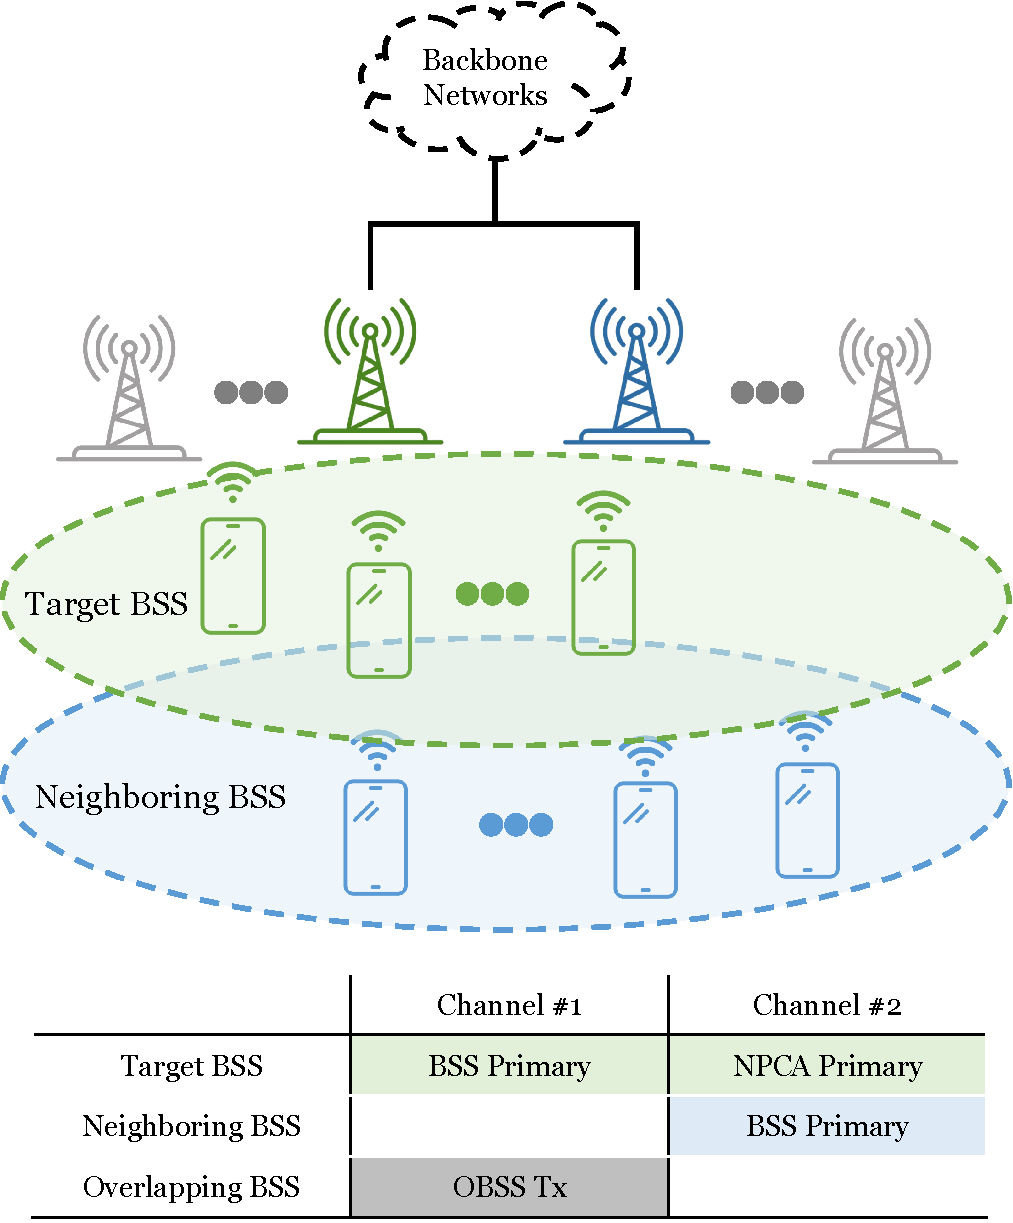
\includegraphics[width=0.45\textwidth]{figure/topology_and_channel.pdf}
    \caption{Two-BSS topology and channel assignment.}
    \label{fig:topology_and_channel}
\end{figure}

Fig.~\ref{fig:topology_and_channel} depicts the two-BSS topology and channel assignment assumed throughout this work. The target BSS, whose NPCA operation is our focus, comprises an Access Point (AP) and a set $\mathcal{N}=\{1,2,\dots,N\}$ of associated non-AP STAs and they can be considered as visitors to the neighboring BSS. The visitors normally contend on their BSS primary channel, Channel~\#1 in Fig.~\ref{fig:topology_and_channel}, which is the main channel used by the target BSS for its own transmissions.

Channel~\#1 is also used by an overlapping BSS (OBSS) operating on the same channel, whose transmissions intermittently render it busy. In standards prior to IEEE 802.11bn, a STA could not initiate a transmission whenever its designated primary channel was busy, even if the secondary channel was idle.
In IEEE 802.11bn, however, the AP can designate a separate channel as the NPCA primary channel, used by the visitors during NPCA operation, named as Channel~\#2 in Fig.~\ref{fig:topology_and_channel}. We use the qualifier ``BSS'' to distinguish the original primary channel from the NPCA primary channel, consistent with P802.11bn Draft terminology~\cite{ieee80211bn}.

The NPCA primary channel is not unused spectrum reserved for the target
BSS: Channel~\#2 is itself the BSS primary channel of the neighboring BSS,
comprising its own AP and a set $\mathcal{M}=\{1,2,\dots,M\}$ of native
STAs that contend on it with standard DCF/EDCA at all times. The visitors,
by contrast, use Channel~\#2 only opportunistically, during NPCA visits.
Two contention disciplines therefore coexist on the NPCA primary channel:
the native STAs' persistent DCF and the visitors' bounded, window-limited
access.

Because the two BSSs only partially overlap in coverage
(Fig.~\ref{fig:topology_and_channel}), the native contention a visitor
experiences on the NPCA primary channel depends on its location. A visitor
inside the overlap region senses, defers to, and competes with the native
STAs, whereas a visitor outside the neighboring BSS coverage encounters no
native traffic there and effectively reuses the channel without contending
with natives. The coexistence cost to the neighboring BSS is thus greatest
when every visitor lies within its coverage. Unless otherwise stated we
adopt this full-overlap configuration---a single collision domain in which
all visitors and native STAs are mutually within carrier-sensing
range---since it upper-bounds the impact on native airtime; the
partial-overlap regime, in which non-overlapping visitors enjoy
interference-free spatial reuse, is left to future work. The resulting
impact on native airtime is evaluated in
Section~\ref{sec:performance_evaluation}.

\begin{figure}
    \centering
    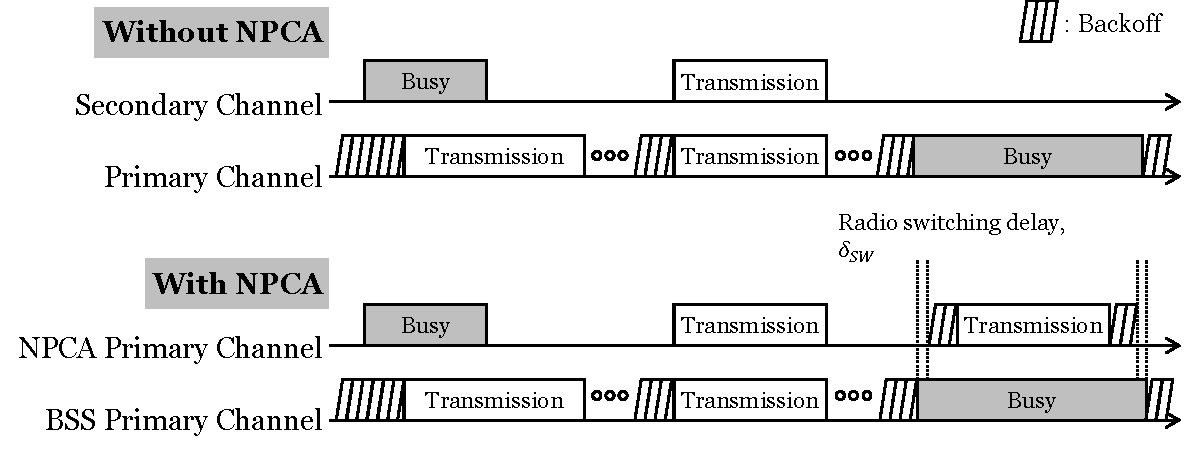
\includegraphics[width=0.48\textwidth]{figure/channel_access.pdf}
    \caption{The medium access process comparison between legacy and NPCA.}
    \label{fig:channel_access}
\end{figure}

\subsection{Legacy versus NPCA Medium Access}
\label{subsec:npca_access}

Let us elaborate on the medium-access process under legacy and NPCA operation.
Fig.~\ref{fig:channel_access} contrasts the two medium-access processes. Under legacy access (top), prior to IEEE 802.11bn, a STA contends only on the BSS primary channel.\footnote{We use the term BSS primary channel to distinguish the original primary channel from the NPCA primary channel introduced in IEEE 802.11bn. Prior to 802.11bn, when NPCA was not yet defined, this channel was referred to simply as the primary channel.} It decrements its backoff counter while the channel is idle and transmits when the counter reaches zero. If the secondary channel is also sensed idle at this instant, the STA may bond it with the BSS primary channel and transmit a wideband PPDU spanning the combined bandwidth (e.g., $40$, $80$, or $160$~MHz). When an overlapping BSS (OBSS) transmission seizes the BSS primary channel, however, the STA must defer and freeze its backoff for the entire OBSS busy period, even though the secondary channel is idle.

Under NPCA access (bottom), a STA no longer wastes the OBSS busy period. When it detects an OBSS transmission on the BSS primary channel, it decodes the preamble of that transmission and learns its duration in advance,\footnote{NPCA relies on preamble detection rather than energy detection: a STA must decode the inter-BSS PPDU preamble (L-SIG and BSS color) at PHY-RXSTART to both classify the transmission and derive its remaining duration, from which the NPCA window is determined. Energy detection alone, which yields no length or BSS information, is insufficient to trigger an NPCA transition.} rather than freezing its backoff for the whole period, it switches to the idle NPCA primary channel and contends and transmits there. On each such switch the STA saves its backoff state on the BSS primary channel and initializes a fresh contention window for the NPCA primary channel, so every NPCA visit begins at the minimum backoff stage regardless of prior history. The STA already knows when the OBSS transmission will finish, so it sets a timer to that instant and switches back to the BSS primary channel when the timer expires, restoring the saved state without having to re-sense the channel. In this way the secondary spectrum that the legacy STA leaves idle is put to use, and a STA can complete one or more transmissions that it would otherwise have had to postpone.

Two constraints shape this access. First, a radio transition delay
$\delta_\mathrm{sw}$ is incurred on each switch. Second, the opportunity
lasts only until the known end of the OBSS transmission, whose remaining
duration $D_\mathrm{rem}$ is read from the preamble. Contention and
transmission must therefore fit within a bounded window of
\begin{equation}
    W_\mathrm{eff} \;=\; \left\lfloor
    \frac{D_\mathrm{rem}-\delta_\mathrm{sw}}{\sigma} \right\rfloor
    \quad\text{slots},
    \label{eq:weff}
\end{equation}
where $\sigma$ is the slot time, typically $9$~$\mu$s in IEEE 802.11-compliance systems. This deadline is the crux of NPCA: every
backoff decision competes against it. A STA that collides doubles its
contention window as usual, and once the resulting backoff exceeds the slots
left in $W_\mathrm{eff}$, it can no longer transmit before the window
closes so it wastes the rest of the opportunity despite having data to send.

Because the contention window is reset at every NPCA visit, this penalty
recurs each time rather than amortizing across visits. This mismatch between
open-ended backoff and the finite window is the inefficiency that PACE
targets.

\subsection{Slotted Contention Model}
\label{subsec:npca_window}

IEEE 802.11 STAs access the medium through the DCF, a CSMA/CA mechanism
in which each STA maintains a backoff counter rather than transmitting
at random in every slot. Directly analyzing DCF over a finite window is
intractable, so we adopt the standard slotted abstraction introduced by
Bianchi~\cite{bianchi2000performance}: the backoff process of a saturated
DCF STA is represented by a single per-slot transmission probability
$\tau$, the steady-state probability that the STA transmits in a
randomly chosen slot. For the standard baseline this is purely an analytical
model of DCF---the mechanism itself remains backoff-based---while $\tau$ also
serves as the per-slot access-probability variable in which we express and
compare the schemes studied here, including the proposed policy of
Section~\ref{sec:pace_algorithm}.

Under this abstraction, we model time on the NPCA primary channel as a
sequence of slots of duration $\sigma$ and index them by
$t\in\{0,1,\dots,W_\mathrm{eff}\}$. We denote by
$W_\mathrm{rem}(t)=W_\mathrm{eff}-t$ the number of slots remaining at slot
$t$, so that $W_\mathrm{rem}$ counts down toward the deadline as contention
proceeds.

Let $\mathcal{V}\subseteq\mathcal{N}$ be the set of STAs that switch to
the NPCA primary channel, each holding a pending PPDU whose transmission
occupies $L_i$ slots. Because a transmission must complete before the
window closes, STA $i$ is viable at slot $t$ only if its frame
still fits, i.e.\ $L_i \le W_\mathrm{rem}(t)$; otherwise it can no longer
succeed and should remain silent to avoid wasting slots. We write the
viable population at slot $t$ as
\begin{equation}
    \mathcal{V}(t) \;=\; \bigl\{\, i\in\mathcal{V} :
    L_i \le W_\mathrm{rem}(t) \,\bigr\},
    \label{eq:viable}
\end{equation}
which is non-increasing in $t$ as both the window depletes and frames
become infeasible.

At each slot, a viable STA $i$ attempts transmission with probability
$\tau_i$. Following the half-duplex assumption, a transmitting STA
cannot sense the channel in the same slot. Let $\mathcal{D}(t)$ denote the
set of STAs whose transmissions on the NPCA primary channel are detected by a
given STA in slot $t$. This set is defined at the channel level: it counts every
STA transmitting on that channel in the slot, not only the switching visitors
but also any other STA that uses the same channel as its own primary. The slot
outcome is idle when $|\mathcal{D}(t)|=0$, a
success when $|\mathcal{D}(t)|=1$, and a collision when
$|\mathcal{D}(t)|\ge 2$. These three observable events are the only
feedback available to a STA, and they drive the adaptive contention
control developed in Section~\ref{sec:pace_algorithm}.

The remaining window advances by the time each outcome occupies the
medium: an idle slot consumes one slot, while a successful slot consumes
$L_\mathrm{solo}(t)$ slots and a collision consumes $L_\mathrm{col}(t)$
slots. The two occupancies depend on the access mode.

\subsubsection{Basic Access}
A successful slot is occupied by the sole sender's frame,
\begin{equation}
    L_\mathrm{solo}(t) \;=\; L_i
    \label{eq:lsolo_basic}
\end{equation}
where $\mathcal{D}(t)=\{i\}$, while a collision keeps the medium busy until the longest colliding frame has ended,
\begin{equation}
    L_\mathrm{col}(t) \;=\; \max_{i\in\mathcal{D}(t)} L_i,
    \label{eq:lmax}
\end{equation}
as in standard IEEE 802.11 without collision detection. Since each STA
holds a single pending PPDU per visit and departs upon success, every
$L_i$ is fixed for the visit's duration; the slot dependence of both
occupancies enters only through the identity of the transmitters
$\mathcal{D}(t)$.

\subsubsection{RTS/CTS-Protected Access}
PACE can also adopt RTS/CTS-protected access, under which the busy-slot
accounting changes. A successful exchange is preceded by the handshake and
therefore occupies
\begin{equation}
    L_\mathrm{solo}(t) \;=\; L_i + L_\mathrm{hs}
    \label{eq:lsolo_rts}
\end{equation}
slots, where $\mathcal{D}(t)=\{i\}$ and
\begin{equation}
    L_\mathrm{hs} \;=\; \left\lceil
    \frac{T_\mathrm{RTS} + T_\mathrm{CTS} + 2\,T_\mathrm{SIFS}}{\sigma}
    \right\rceil
    \label{eq:oh_rts}
\end{equation}
is the handshake overhead, with $T_\mathrm{RTS}$, $T_\mathrm{CTS}$, and
$T_\mathrm{SIFS}$ being the respective durations defined in IEEE 802.11. A collision, by
contrast, involves only RTS frames: the data frames are never sent, and
the channel recovers after the extended interframe space, so a collision
occupies
\begin{equation}
    L_\mathrm{col} \;=\; \left\lceil
    \frac{T_\mathrm{RTS} + T_\mathrm{EIFS}}{\sigma} \right\rceil
    \label{eq:coll_rts}
\end{equation}
slots, where $T_\mathrm{EIFS}=T_\mathrm{SIFS}+T_\mathrm{ACK}+T_\mathrm{DIFS}$
is the extended interframe space. Unlike its basic-access counterpart
of~\eqref{eq:lmax}, this occupancy is a constant, independent of the
colliding frame lengths and of the slot index. Under protection the viability test of~\eqref{eq:viable} must also leave room for the handshake, i.e.\ $L_i$
is replaced by $L_i+L_\mathrm{hs}$. Basic access is recovered as the
special case $L_\mathrm{hs}=0$ with $L_\mathrm{col}(t)$ given
by~\eqref{eq:lmax}.

We set RTS/CTS-Protected Access as the default for three reasons. First, it bounds the cost of a
collision to the constant $L_\mathrm{col}$ of~\eqref{eq:coll_rts} instead of a full frame length,
which is precisely the premise under which the probabilistic target of
Section~\ref{sec:pace_algorithm} is throughput-optimal. Second, the RTS/CTS
control frames, sent at a robust base rate, are the natural carrier of the
advertised probability that PACE's feedback rule copies on solo successes.
Third, RTS/CTS protects visits under the hidden-terminal conditions typical
of OBSS environments, beyond the single-collision-domain model adopted
here. Both modes are evaluated in
Section~\ref{subsec:eval_whypace}.

\begin{figure}
    \centering
    \begin{subfigure}{\linewidth}
        \centering
        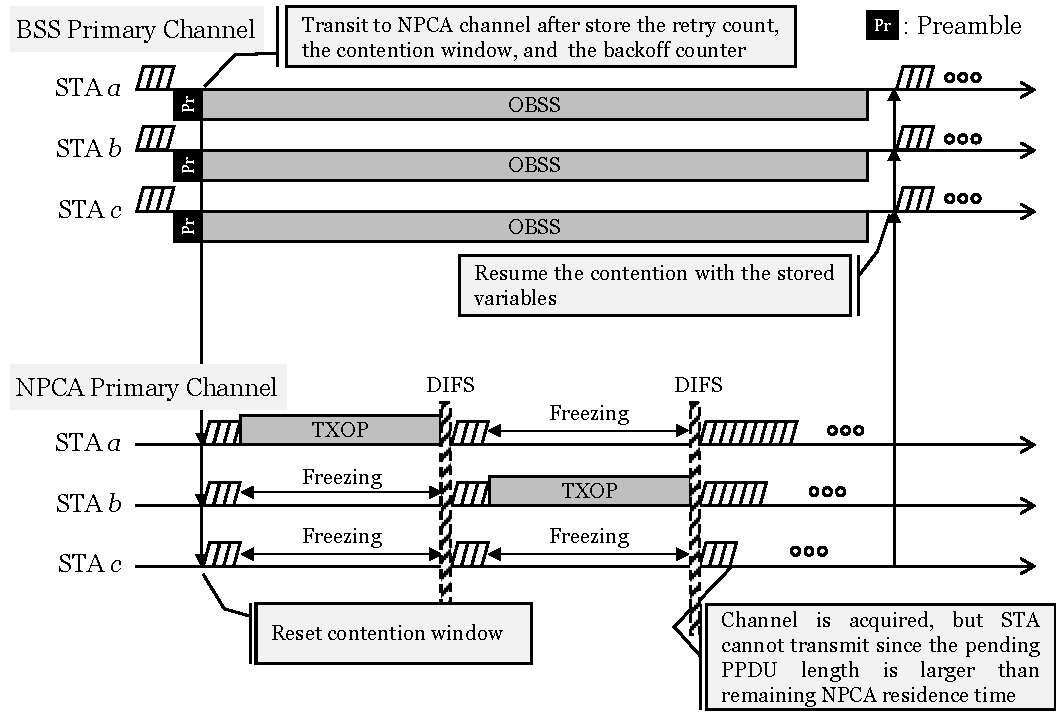
\includegraphics[width=\linewidth]{figure/transition_npca.pdf}
        \caption{NPCA baseline (binary exponential backoff).}
        \label{fig:transition_npca}
    \end{subfigure}
    \\[1.5ex]
    \begin{subfigure}{\linewidth}
        \centering
        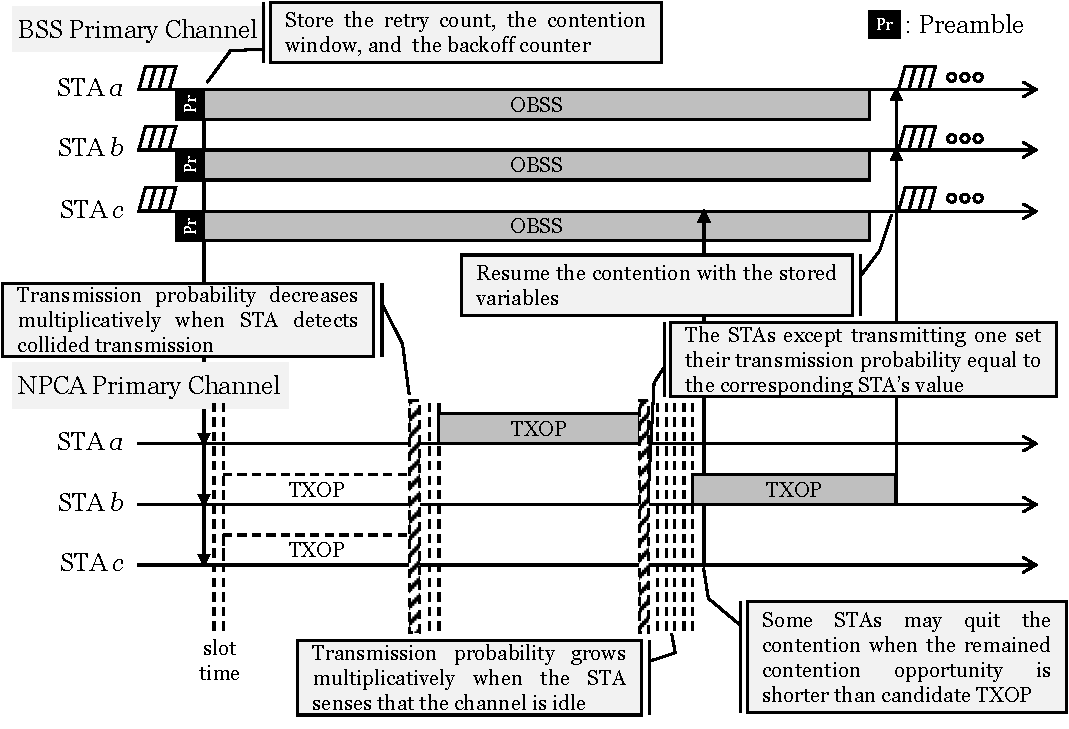
\includegraphics[width=\linewidth]{figure/transition_pace.pdf}
        \caption{Proposed PACE (probabilistic adaptive contention).}
        \label{fig:transition_pace}
    \end{subfigure}
    \caption{Medium access on the NPCA primary channel: a STA that detects
    an OBSS transmission on the BSS primary channel migrates and contends within
    the bounded NPCA window. (a) the standard NPCA baseline with binary
    exponential backoff, and (b) the proposed PACE with probabilistic adaptive
    contention and PPDU-aware self-exclusion.}
    \label{fig:contention}
\end{figure}

Fig.~\ref{fig:contention} illustrates this slotted contention on the NPCA primary channel and contrasts the two schemes studied in this paper. In both, a STA that detects an OBSS transmission on the BSS primary channel stores its DCF state, migrates to the NPCA primary channel, and contends there until the NPCA timer expires, whereupon it restores the saved state and resumes on the BSS primary channel. Under the NPCA baseline of Fig.~\ref{fig:transition_npca}, STAs contend with binary exponential backoff (BEB), that is, a STA that collides doubles its contention window, and one whose pending TXOP no longer fits the remaining window acquires the channel only to find it cannot transmit, wasting the slots it occupied. 

Meanwhile, under the proposed PACE scheme of Fig.~\ref{fig:transition_pace}, each STA instead adapts its per-slot probability $\tau_i$ from the idle, success, and collision feedback. The access probability is raised multiplicatively on idle slots, lowered on collisions, and replaced by the successful sender's value on solo receptions. In addition, a STA proactively withdraws from contention once its frame can no longer fit within $W_\mathrm{rem}(t)$. We detail this mechanism in Section~\ref{sec:pace_algorithm}.

\section{PACE Algorithm}
\label{sec:pace_algorithm}

\begin{algorithm}[t]
\caption{PACE at STA $i$ during one NPCA visit}
\label{alg:pace}
\begin{algorithmic}[1]
\REQUIRE PPDU length $L_i$ (slots), window $W_\mathrm{eff}$, factors $c_\mathrm{coll},\,c_\mathrm{idle}>1$, handshake overhead $L_\mathrm{hs}$ of Eq.~\eqref{eq:oh_rts} ($L_\mathrm{hs}=0$ under basic access)
\PHASE {/* Phase (a): Probability Initialization */}
\STATE $\tau_i \leftarrow 1/W_\mathrm{eff}$;\quad $W_\mathrm{rem} \leftarrow W_\mathrm{eff}$
\WHILE{$W_\mathrm{rem} > 0$}
    \PHASE {/* Phase (b): PPDU-aware Self-Exclusion */}
    \IF{$L_i + L_\mathrm{hs} > W_\mathrm{rem}$}
        \STATE $\tau_i \leftarrow 0$
    \ENDIF
    \PHASE {/* Phase (c): Probabilistic Channel Access */}
    \STATE draw $u \sim \mathrm{Uniform}(0,1)$
    \IF{$u < \tau_i$}
        \STATE exchange RTS/CTS, then transmit the PPDU, advertising $\tau_i$
        \IF{solo success}
            \STATE \textbf{break}
        \ENDIF
        \STATE $W_\mathrm{rem} \leftarrow W_\mathrm{rem} - L_\mathrm{col}(t)$ \COMMENT{collided: Eq.~\eqref{eq:coll_rts} under protection, Eq.~\eqref{eq:lmax} under basic access}
    \ELSE
        \PHASE {/* Phase (d): Feedback-based Adaptation */}
        \STATE observe the slot outcome $|\mathcal{D}(t)|$
        \IF{$|\mathcal{D}(t)| = 0$}
            \STATE $\tau_i \leftarrow \min(\tau_i \cdot c_\mathrm{idle},\;1)$;\quad $W_\mathrm{rem} \leftarrow W_\mathrm{rem} - 1$
        \ELSIF{$|\mathcal{D}(t)| = 1$}
            \STATE $\tau_i \leftarrow \tau_\mathrm{sender}$;\quad $W_\mathrm{rem} \leftarrow W_\mathrm{rem} - L_\mathrm{solo}(t)$
        \ELSE
            \STATE $\tau_i \leftarrow \tau_i / c_\mathrm{coll}$;\quad $W_\mathrm{rem} \leftarrow W_\mathrm{rem} - L_\mathrm{col}(t)$
        \ENDIF
    \ENDIF
\ENDWHILE
\end{algorithmic}
\end{algorithm}

Algorithm~\ref{alg:pace} summarizes PACE as executed independently by each STA on the NPCA primary channel during a single NPCA visit. Every STA runs the same rule using only locally observable feedback, those are, the per-slot outcome and its own remaining window without central coordination or knowledge of the contending population.

Algorithm~\ref{alg:pace} is expressed in the per-slot transmission-probability
model of Section~\ref{subsec:npca_window}: a viable STA transmits in a slot
with probability $\tau_i$. This is a probabilistic, slotted-ALOHA-style access
policy.

We adopt the probabilistic approach for two reasons. First, the
per-slot probability $\tau$ is the common abstraction under which DCF, PND, and
AND are all analyzed~\cite{bianchi2000performance,song2014pnd,vasudevan2013efficient},
so it places PACE on the same analytical footing as the baselines we compare
against. Second, and more fundamentally, the finite NPCA window is precisely
where a deterministic countdown breaks down: a single backoff draw cannot
re-adapt within the handful of slots a visit lasts, whereas a per-slot
probability can be re-steered every slot by the feedback law, which will be described in Subsec.~\ref{subsec:adaptive_control}. The
ALOHA-style attempt is therefore not incidental but the mechanism that makes
within-window adaptation possible.

Algorithm~\ref{alg:pace} runs four phases per visit: (a) a one-time probability
initialization, followed by a per-slot loop of (b) self-exclusion, (c) channel
access, and (d) feedback-based adaptation. The remainder of this section develops
each phase in turn.

\subsection{Probability Initialization}
\label{subsec:init}

A visitor that has just switched to the NPCA primary channel does not know how
many other STAs are contending there. The population-matched choice
$\tau_0=1/N$, which is the well-known throughput-optimal attempt probability of
slotted ALOHA, is therefore unavailable in practice since $N$ is not observable.

Visitor STAs might, through association state or management traffic, form some
estimate of how many STAs belong to its own BSS. The harder obstacle is that
the population it actually contends with also includes the native STAs of the
neighboring BSS that owns the NPCA primary channel. That is, a visitor competes against these as well, yet has no direct way to learn how many are active. The count that would
parameterize $1/N$ is thus doubly hidden, which motivates a surrogate that
avoids counting STAs altogether.

We propose a method where the window length itself determines the scale. A visit spans $W_\mathrm{eff}$ slots, and a STA contends in at most one of them per slot so $W_\mathrm{eff}$ upper-bounds the number of attempt opportunities any STA sees in a visit. A STA attempting with probability $\tau$ therefore expects at most $W_\mathrm{eff}\,\tau$ attempts before the deadline. Fixing this budget to a single probe per STA,
\begin{equation}
    W_\mathrm{eff}\,\tau_0 = 1,
    \label{eq:one_probe}
\end{equation}
sets the most conservative self-consistent  exploration rate: low enough to avoid an early collision storm, yet high enough for each STA to test the medium about once before the window drains. This yields
\begin{equation}
    \tau_0 = \frac{1}{W_\mathrm{eff}},
    \label{eq:init}
\end{equation}
which depends only on the effective window $W_\mathrm{eff}$, which is a quantity that each STA can compute locally from the OBSS PPDU duration. No knowledge of the contender count is required.

In general frame length to be transmitted on NPCA primacy channel is longer than a single slot, so $\tau_0 $ is bound to be smaller than the optimal value. This choice is deliberately biased toward under-attempting for two reasons. First, it is self-correcting in the safe direction: an over-conservative $\tau_i$ is raised toward the operating point within a few slots by the idle-driven multiplicative increase in Phase~(d), whereas an over-aggressive start triggers collisions whose wasted slots cannot be reclaimed inside a finite window. The MIMD recovery is thus asymmetric, and starting low pays only a bounded ramp-up cost. Second, $1/W_\mathrm{eff}$ tracks the regime where initialization matters most: when the window is tight ($W_\mathrm{eff}\!\approx\!N$) it already approximates the optimum $1/N$, and when the window is loose ($W_\mathrm{eff}\!\gg\!N$) the mild initial timidity is erased by the idle increase long before the window drains. 
% Section~\ref{sec:performance_evaluation} shows that this locally computable initialization stays within a few percent of the count-aware optimum across the entire window-tightness range, while aggressive or wide-spread initializations collapse---confirming that PACE inherits the initialization-robustness of neighbor discovery only when the initial scale is kept at or below $1/W_\mathrm{eff}$.

\subsection{PPDU-aware Self-Exclusion}
\label{subsec:self_exclusion}

At the start of every slot a STA compares its own frame length $L_i$ to the remaining window $W_\mathrm{rem}(t)$. If $L_i > W_\mathrm{rem}(t)$ the frame can no longer finish before the deadline, so the STA sets $\tau_i=0$ and falls silent for the rest of the visit. The test is purely local. That means it involves only the STA's own $L_i$ and the slot index and thus, like initialization, requires no knowledge of the contending population.

Self-exclusion keeps the optimal target that PACE aims to track,
\begin{equation}
    \tau^*(t) \;=\; \frac{1}{|\mathcal{V}(t)|},
    \label{eq:tau_opt}
\end{equation}
meaningful in a heterogeneous and finite window. In a slot with $|\mathcal{V}(t)|$ viable STAs, a success, meaning exactly one transmitter, is most likely when each attempts with probability $\tau^*(t)$, and this target rises over the visit as the viable set drains. A STA whose frame no longer fits is removed from the viable set $\mathcal{V}(t)$ of Eq.~\eqref{eq:viable}, so it neither wastes time on attempts destined to fail nor inflates the contention seen by the STAs that can still succeed. This plays the same role as the collision detection departure of the original neighbor discovery algorithm, in which a STA leaves the contention once its advertisement succeeds. Here a STA also leaves once its frame provably cannot complete, tightening $\mathcal{V}(t)$ toward the set of STAs that genuinely compete for the remaining slots.

\subsection{Probabilistic Channel Access}
\label{subsec:channel_access}

A STA that is still viable transmits in the current slot with probability $\tau_i$ and otherwise listens. Because the radio is half-duplex, a transmitting STA cannot sense the slot it occupies, so it performs no adaptation on its own transmissions. Each transmitted PPDU advertises the sender's current $\tau_i$ in its header, which the listeners use in Phase~(d).

A slot is a success when exactly one viable STA transmits and its frame fits the remaining window. The winner then departs the visit---mirroring the post-success departure of neighbor discovery---which decrements $|\mathcal{V}(t)|$ and raises the optimal target $\tau^*(t)$ for the STAs that remain. Slots with no transmission are idle, and slots with two or more transmissions are collisions; both outcomes are observed by every non-transmitting STA and feed the adaptation of Phase~(d).

\subsection{Feedback-based Adaptation}
\label{subsec:adaptive_control}

Every viable STA that listened in the slot updates $\tau_i$ from the slot outcome $|\mathcal{D}(t)|$ using the multiplicative-increase and multiplicative-decrease (MIMD) rule inherited from neighbor discovery as
\begin{equation}
\tau_i \leftarrow
\begin{cases}
\min(c_\mathrm{idle}\,\tau_i,\,1) & |\mathcal{D}(t)|=0 \quad(\text{idle}),\\[2pt]
\tau_\mathrm{sender}              & |\mathcal{D}(t)|=1 \quad(\text{solo success}),\\[2pt]
\tau_i / c_\mathrm{coll}          & |\mathcal{D}(t)|\ge 2 \quad(\text{collision}),
\end{cases}
\label{eq:mimd}
\end{equation}
with $c_\mathrm{idle},c_\mathrm{coll}>1$. 

An idle slot signals that the
population has been overestimated and the attempt rate is raised by the factor of $c_\mathrm{idle}$. On the other hand, a collision signals the opposite, hence, once STAs detect a collision, the attempt rate is divided by $c_\mathrm{coll}$ to reduce the contention. On a solo success, every listener copies the advertised $\tau_\mathrm{sender}$, so a single successful slot propagates the winning operating point to the whole contending set at once, giving PACE the fast intra-visit consensus.

None of the three updates counts the viable STAs. Instead, the idle and collision statistics move each $\tau_i$ toward the operating point implicitly, and solo-copy pulls the population onto a common value, so the ensemble approximately tracks the time-varying optimum $\tau^*(t)$ of Eq.~\eqref{eq:tau_opt} without estimating the number of contending STAs $|\mathcal{V}(t)|$. 

The direction of this adaptation is what separates PACE from legacy binary exponential backoff (BEB). Because the viable set only shrinks over a visit, the optimal target $\tau^*(t)=1/|\mathcal{V}(t)|$ of~\eqref{eq:tau_opt} rises as the deadline approaches. On the other hand, the BEB moves the opposite way, that is, a collision doubles the contention window and halves the attempt rate, so the access probability falls exactly when it should climb.

Finally, the rule of Eq.~\eqref{eq:mimd} needs no modification to operate alongside the native STAs of Section~\ref{subsec:network_model}. Because the slot outcome $\mathcal{D}(t)$ is measured at the channel level, native activity enters a visitor's feedback directly: a slot in which two or more frames overlap is a collision whether the extra transmitter is a visitor or a native, so a native transmission that clashes with a visitor lowers that visitor's $\tau_i$, and a slot with no transmission at all, native or visitor, is idle and raises it. The solo case is the one exception. The copy $\tau_i \leftarrow \tau_\mathrm{sender}$ requires the successful frame to advertise a probability, which only a PACE visitor does; when a native transmits alone, its frame carries no such value, so a listening visitor keeps $\tau_i$ unchanged and simply observes the busy slot while the window continues to shrink.

% The mismatch is twofold. First, the adaptation is backwards---BEB retreats on congestion while the window's diminishing population
% calls for a more aggressive attempt rate---so late slots are left idle. Second,
% the doubled backoff can exceed the remaining window $W_\mathrm{rem}(t)$,
% silencing the STA for the rest of the visit and wasting those slots
% outright; unlike PACE's self-exclusion, which silences only STAs that
% provably cannot finish, this dead time falls on STAs that could still have
% succeeded. PACE's idle-increase and solo-copy instead move $\tau_i$ along the
% rising $\tau^*(t)$ trajectory, matching the sign of the optimal policy rather
% than fighting it.

\section{Performance Evaluation}
\label{sec:performance_evaluation}

\begin{table}[t]
\centering
\caption{Simulation Parameters}
\label{tab:sim_params}
\begin{tabular}{ll}
\hline
\textbf{Parameter} & \textbf{Value} \\
\hline
Visitor STAs $N$ (scheme under test) & $\{5, 10, 20, 50\}$ \\
Native STAs $M$ (always standard DCF) & $10$ \\
Slot time $\sigma$ / SIFS / DIFS  & $9$ / $16$ / $34~\mu$s \\
Effective window $W_\mathrm{eff}$ & $420$ slots ($3.78$~ms) \\
Visitor PPDU duration            & $\mathcal{U}[225, 900]~\mu$s \\
Native PPDU duration             & $450~\mu$s \\
Initial probability $\tau_0$     & $1/W_\mathrm{eff}$ \\
MIMD factors $c_\mathrm{coll},c_\mathrm{idle}$ & $1.2$ \\
$\mathrm{CW}_{\min}$ / $\mathrm{CW}_{\max}$ for BEB & $15$ / $1023$ \\
RTS/CTS $L_\mathrm{hs}$ / $L_\mathrm{col}$ (24~Mbps ctrl.) & $88$ / $106~\mu$s \\
Transitions $\times$ sequences $\times$ seeds & $50 \times 20 \times 5$ \\
\hline
\end{tabular}
\end{table}

We evaluate PACE in the slotted NPCA contention model of
Section~\ref{subsec:npca_window} under IEEE~802.11 OFDM timing;
Table~\ref{tab:sim_params} summarizes the parameters. A visit spans
$W_\mathrm{eff}=3.78$~ms ($420$ slots of $\sigma=9~\mu$s), contended by
$N\in\{5,10,20,50\}$ visitor STAs running the scheme under test alongside
$M=10$ native STAs that always run standard DCF. Visitor PPDU durations
are drawn uniformly from $225$--$900~\mu$s and native frames last
$450~\mu$s. PACE follows Algorithm~\ref{alg:pace} with
$\tau_0=1/W_\mathrm{eff}$ and $c_\mathrm{coll}=c_\mathrm{idle}=1.2$; the
standard-compliant baseline contends with CSMA/CA
($\mathrm{CW}_{\min}=16$, binary exponential backoff, NPCA
minimum-duration check); and the oracle transmits at
$\tau^*(t)=1/|\mathcal{V}(t)|$ with perfect knowledge of the viable set.
Both access modes of Section~\ref{subsec:npca_window} are evaluated:
basic access, in which a collision is charged the longest colliding
frame, eq.~\eqref{eq:lmax}, and mandatory RTS/CTS with the
standard-derived costs $L_\mathrm{hs}=88~\mu$s and
$L_\mathrm{col}=106~\mu$s. Each data point averages the steady half of
$50$ consecutive NPCA transitions over $20$ sequences and five seeds.
Performance is reported as the total useful airtime of the channel
normalized by $W_\mathrm{eff}$, its split between visitors and natives,
and the visitor airtime proportionality index defined in
Section~\ref{subsec:eval_fairness}.

\subsection{Why PACE: Channel Airtime under Mixed Contention}
\label{subsec:eval_whypace}

\begin{figure}[t]
    \centering
    \begin{subfigure}[b]{\columnwidth}
        \centering
        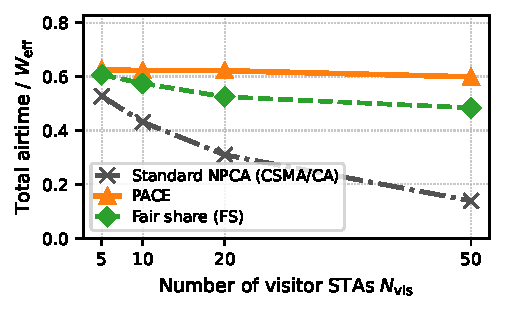
\includegraphics[width=\linewidth]{figure/fig1-1_total.pdf}
        \caption{Basic access (no RTS/CTS).}
        \label{fig:why_pace_basic}
    \end{subfigure}
    \vspace{0.6em}

    \begin{subfigure}[b]{\columnwidth}
        \centering
        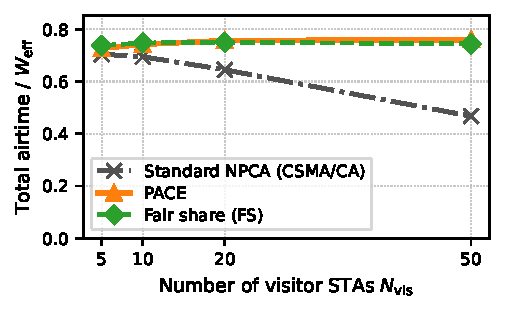
\includegraphics[width=\linewidth]{figure/fig1-2_total.pdf}
        \caption{Mandatory RTS/CTS.}
        \label{fig:why_pace_rts}
    \end{subfigure}
    \caption{Total useful airtime (visitor and native combined) versus the
    number of visitor STAs $N$ for standard-compliant NPCA (CSMA/CA
    visitors), PACE, and the oracle, in the mixed native/visitor channel
    with $M=10$ native DCF stations, under IEEE~802.11 timing
    ($W_\mathrm{eff}=3.78$~ms, visitor PPDU $225$--$900~\mu$s, native PPDU
    $450~\mu$s).}
    \label{fig:why_pace}
\end{figure}

We first ask the question that motivates this work: what does PACE buy over
simply running the standard access procedure on the non-primary channel?
The design objective of PACE is not visitor throughput per se, but to keep
the shared NPCA channel \emph{efficient and fair}: the oracle
$\tau^*(t)=1/|\mathcal{V}(t)|$, computed over \emph{all} contenders, is
precisely the embodiment of that objective, and the evaluation therefore
reports the \emph{total} useful airtime of the channel.
Fig.~\ref{fig:why_pace} compares $N\in\{5,\dots,50\}$ visitor STAs
operating either standard CSMA/CA ($\mathrm{CW}_{\min}=16$, binary
exponential backoff, with the NPCA minimum-duration check) or PACE exactly
as specified in Algorithm~\ref{alg:pace}---every visit starts cold from
$\tau_0=1/W_\mathrm{eff}$---sharing the channel with $M=10$ native DCF
stations, using IEEE~802.11 OFDM timing ($\sigma=9~\mu$s).

Under basic access (Fig.~\ref{fig:why_pace_basic}), the channel under
standard-compliant visitors degrades monotonically as the visitor
population grows, from $0.51$ at $N=5$ to $0.14$ at $N=50$: the fixed
$\mathrm{CW}_{\min}=16$ is far below the contention level, collisions
cascade---each charged the full length of the longest colliding
frame---and the visitors drag natives down with them. The standard
procedure thus does not merely starve the visitors; it destroys the
channel. PACE instead holds the total airtime essentially flat at
$0.64$--$0.70$ across the entire range, $4.7\times$ the standard procedure
at $N=50$. The composition behind this flat total is the fair-sharing
behavior by design: at $N=5$ the deliberately timid start
$\tau_0=1/W_\mathrm{eff}$ leaves the channel largely to the natives
(visitor share $0.06$), and as the visitor population---and hence its
legitimate demand---grows, the idle-driven increase raises the visitors'
share monotonically to $0.52$ at $N=50$, while self-exclusion returns
slots that can no longer carry a full frame. PACE even exceeds the oracle
in total airtime here, because the oracle enforces the per-STA fair
attempt rate at the cost of collisions that basic access charges at full
frame length, whereas PACE's conservative ramp avoids them.

Under the default RTS/CTS-protected mode (Fig.~\ref{fig:why_pace_rts}),
a collision costs the constant $L_\mathrm{col}$ of Eq.~\eqref{eq:coll_rts}
($106~\mu$s) instead of a full frame, at the price of the $L_\mathrm{hs}$
handshake ($88~\mu$s) on every success. Collisions being cheap, the
fair-share oracle is now also airtime-optimal, and PACE tracks it within
$2\%$ over the whole range ($0.70$--$0.74$), while the channel under
standard visitors still declines from $0.67$ to $0.45$ as the
frozen-backoff pathology persists---leaving PACE with $65\%$ more channel
airtime at $N=50$. Taken together, the two panels justify PACE's premise:
inside a finite NPCA window shared with natives, probabilistic
deadline-aware access keeps the channel near its efficient-and-fair
operating point where the standard backoff either idles or collides it
away.

\subsection{Fairness between Natives and Visitors}
\label{subsec:eval_fairness}

\begin{figure}[t]
    \centering
    \begin{subfigure}[b]{\columnwidth}
        \centering
        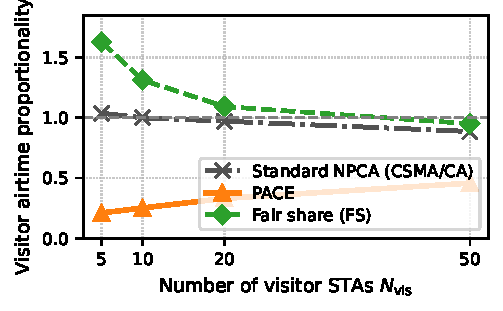
\includegraphics[width=\linewidth]{figure/fig2-1.pdf}
        \caption{Basic access (no RTS/CTS).}
        \label{fig:fairness_basic}
    \end{subfigure}
    \vspace{0.6em}

    \begin{subfigure}[b]{\columnwidth}
        \centering
        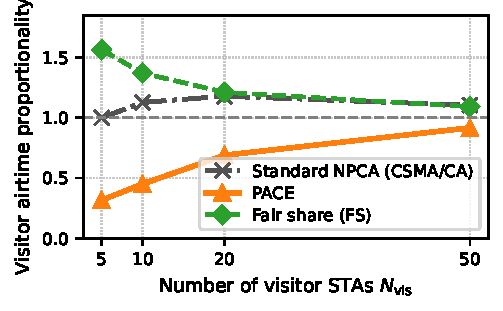
\includegraphics[width=\linewidth]{figure/fig2-2.pdf}
        \caption{Mandatory RTS/CTS.}
        \label{fig:fairness_rts}
    \end{subfigure}
    \caption{Visitor airtime proportionality
    $\rho=\bigl(\text{visitor airtime share}\bigr)/\bigl(N/(N+M)\bigr)$
    versus the number of visitor STAs $N$, in the same setting as
    Fig.~\ref{fig:why_pace}. $\rho=1$ is the proportional-fair reference;
    $\rho>1$ means the visitors occupy more than their population share.}
    \label{fig:fairness}
\end{figure}

Total airtime alone does not reveal who receives it, so we next examine
how the window is divided between the two populations.
Fig.~\ref{fig:fairness} reports the visitor airtime proportionality index
$\rho$, the visitors' share of the useful airtime normalized by their
population share $N/(N+M)$, in the identical setting as
Fig.~\ref{fig:why_pace}: $\rho=1$ is proportional fairness, and
$\rho>1$ indicates that the visitors occupy the channel beyond their
share.

The oracle itself sits well above unity ($\rho=1.7$ at $N=5$, falling to
$1.1$ at $N=50$), which calibrates the reference: even a per-STA fair
attempt rate yields a visitor-leaning split, both because the visitor
frames are longer than the native ones ($562~\mu$s versus $450~\mu$s on
average) and because the natives' DCF decrements its backoff only in idle
slots and therefore competes sluggishly inside a busy window. Exact
proportionality is thus not attainable by any attempt-fair policy in this
setting, and the oracle curve marks the practically fair operating line.

Against this reference the two schemes separate cleanly. The
standard-compliant visitors hold $\rho\approx 1.1$--$1.25$ throughout:
they take more than their population share even while, as
Fig.~\ref{fig:why_pace_basic} showed, their collision cascades destroy
the channel at large $N$---the worst of both worlds, over-proportional
and inefficient. PACE instead operates \emph{below} unity across the
entire range and approaches proportionality from beneath as the visitor
demand grows ($\rho$ rising from $0.26$ to $0.93$ under basic access and
from $0.37$ to $0.97$ under RTS/CTS). This is the fairness counterpart of
the flat total-airtime curves of Fig.~\ref{fig:why_pace}: the
conservative start $\tau_0=1/W_\mathrm{eff}$ concedes the channel to the
natives when few visitors are present, and the idle-driven increase
claims airtime only as the visitor population---and hence its legitimate
share---grows. PACE therefore never extracts its gain from the natives:
its advantage over the standard procedure in
Section~\ref{subsec:eval_whypace} comes from slots that contention had
been wasting, not from native airtime.

\section{Conclusion}
\label{sec:conclusion}
\blindtext



\bibliographystyle{IEEEtran}
\bibliography{pace}

\end{document}
